\documentclass[12pt]{article} 
\usepackage[utf8]{inputenc}
\usepackage[T1]{fontenc} 
\usepackage[portuguese]{babel} 
\usepackage{tikz}
\usepackage{graphicx}
\usepackage{hyperref} 
\usepackage{booktabs} 
\usepackage{footnote}
\usepackage{url}
\usepackage{amsmath}
\usepackage{geometry} 
\geometry{a4paper, margin=1in}

\interfootnotelinepenalty=10000

\title{Relatório de Análise de Série Temporal no Mercado Imobiliário}
\author{Gabriel Fruet} \date{\today}

\begin{document}

\maketitle

\section{Introdução} Este relatório apresenta uma análise da série temporal da
razão de consumidores entre 38 e 58 anos em relação ao número de empresas
ativas por estado, no período de 2007 a 2022. Utilizei dados da SCOD Brasil e
do IBGE para realizar esta análise.

\section{Metodologia} 

\subsection{Coleta de Dados} 

Os dados das empresas foram
obtidos da Tabela 1757 do SIDRA, utilizando requisições HTTP diretamente
através da biblioteca \texttt{requests}, sem o uso de bibliotecas prontas como
\texttt{sidrapy}. 

Para obter os dados do SIDRA, utilizei a URL 
\footnote{\url{https://apisidra.ibge.gov.br/values/t/1757/n2/all/p/2007-2020}}
 A interpretação
dessa URL é esta: Consulte no SIDRA os valores da Tabela 1757, para todos os
componentes do  nível territorial n2 (Grande Região) entre os anos de 2007 e
2020

A população estimada foi obtida da projeção populacional
disponibilizada pelo IBGE, através da URL 
\footnote{\url{https://ftp.ibge.gov.br/Projecao_da_Populacao/Projecao_da_Populacao_2024/projecoes_2024_tab1_idade_simples.xlsx}}.


\subsection{Tendência dos dados}

\begin{figure}[!htbp]
    \begin{center}
    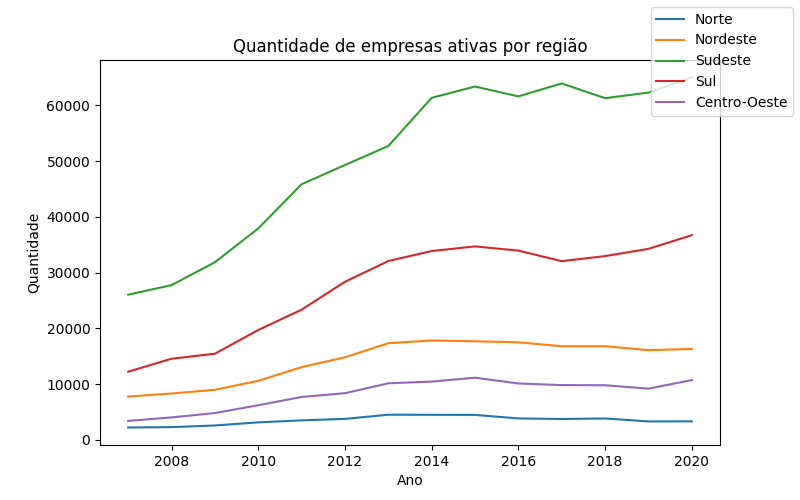
\includegraphics[width=0.7\textwidth]{../figures/time_series_business.png}
    \caption{\label{fig:trend_bus} Comportamento da quantidade de empresas ativas por ano}
    \end{center}
\end{figure}

\begin{figure}[!htbp]
    \begin{center}
    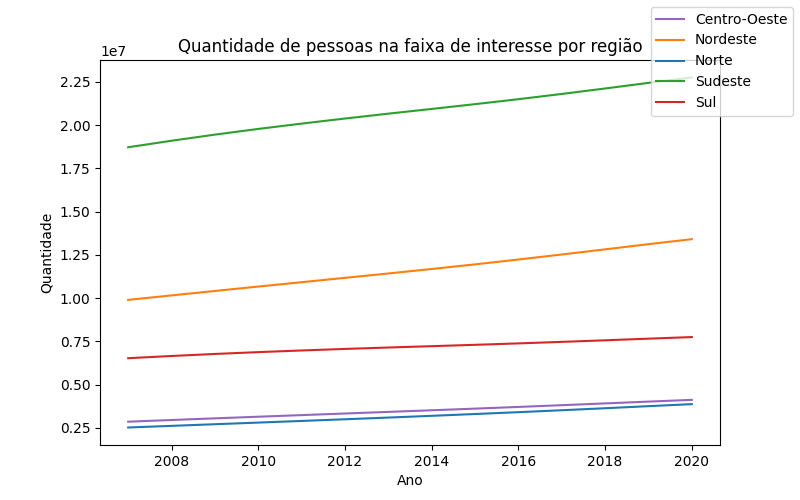
\includegraphics[width=0.7\textwidth]{../figures/time_series_population.png}
    \caption{\label{fig:trend_pop} Comportamento da população entre 38 e 58 anos por ano}
    \end{center}
\end{figure}

\begin{figure}[!htbp]
    \begin{center}
    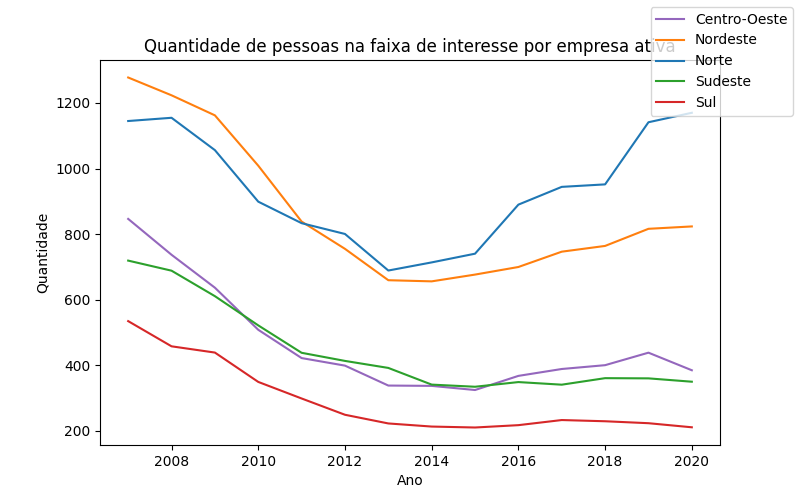
\includegraphics[width=0.7\textwidth]{../figures/time_series_ratio.png}
    \caption{\label{fig:trend_rat} Comportamento da quantidade de pessoas na faixa de interesse por empresas ativas por ano}
    \end{center}
\end{figure}

Como podemos ver na fígura \ref{fig:trend_pop}, a população vem aumentando
desde 2008. Ademais, de acordo com a fígura \ref{fig:trend_bus}, a quantidade
de empresas ativas no setor de construção também têm aumentado desde 2008,
apesar de uma leve desaceleração em torno de 2014, possivelmente devido à crise
que o país sofreu.

Ao combinar esses dados em uma razão, percebemos que através da fígura
\ref{fig:trend_rat} a tendência no período de 2014, foi uma diminuição na
demanda por empresas do ramo de construção, possivelmente devido a falência de
empresas, já que a população não costuma diminuir bruscamente. Porém, houve um aumento
e retorno significativo, especialmente após 2016 na Grande Região Norte.



\subsection{Analise de Estacionaridade} 

\begin{figure}[!htbp]
    \begin{center}
    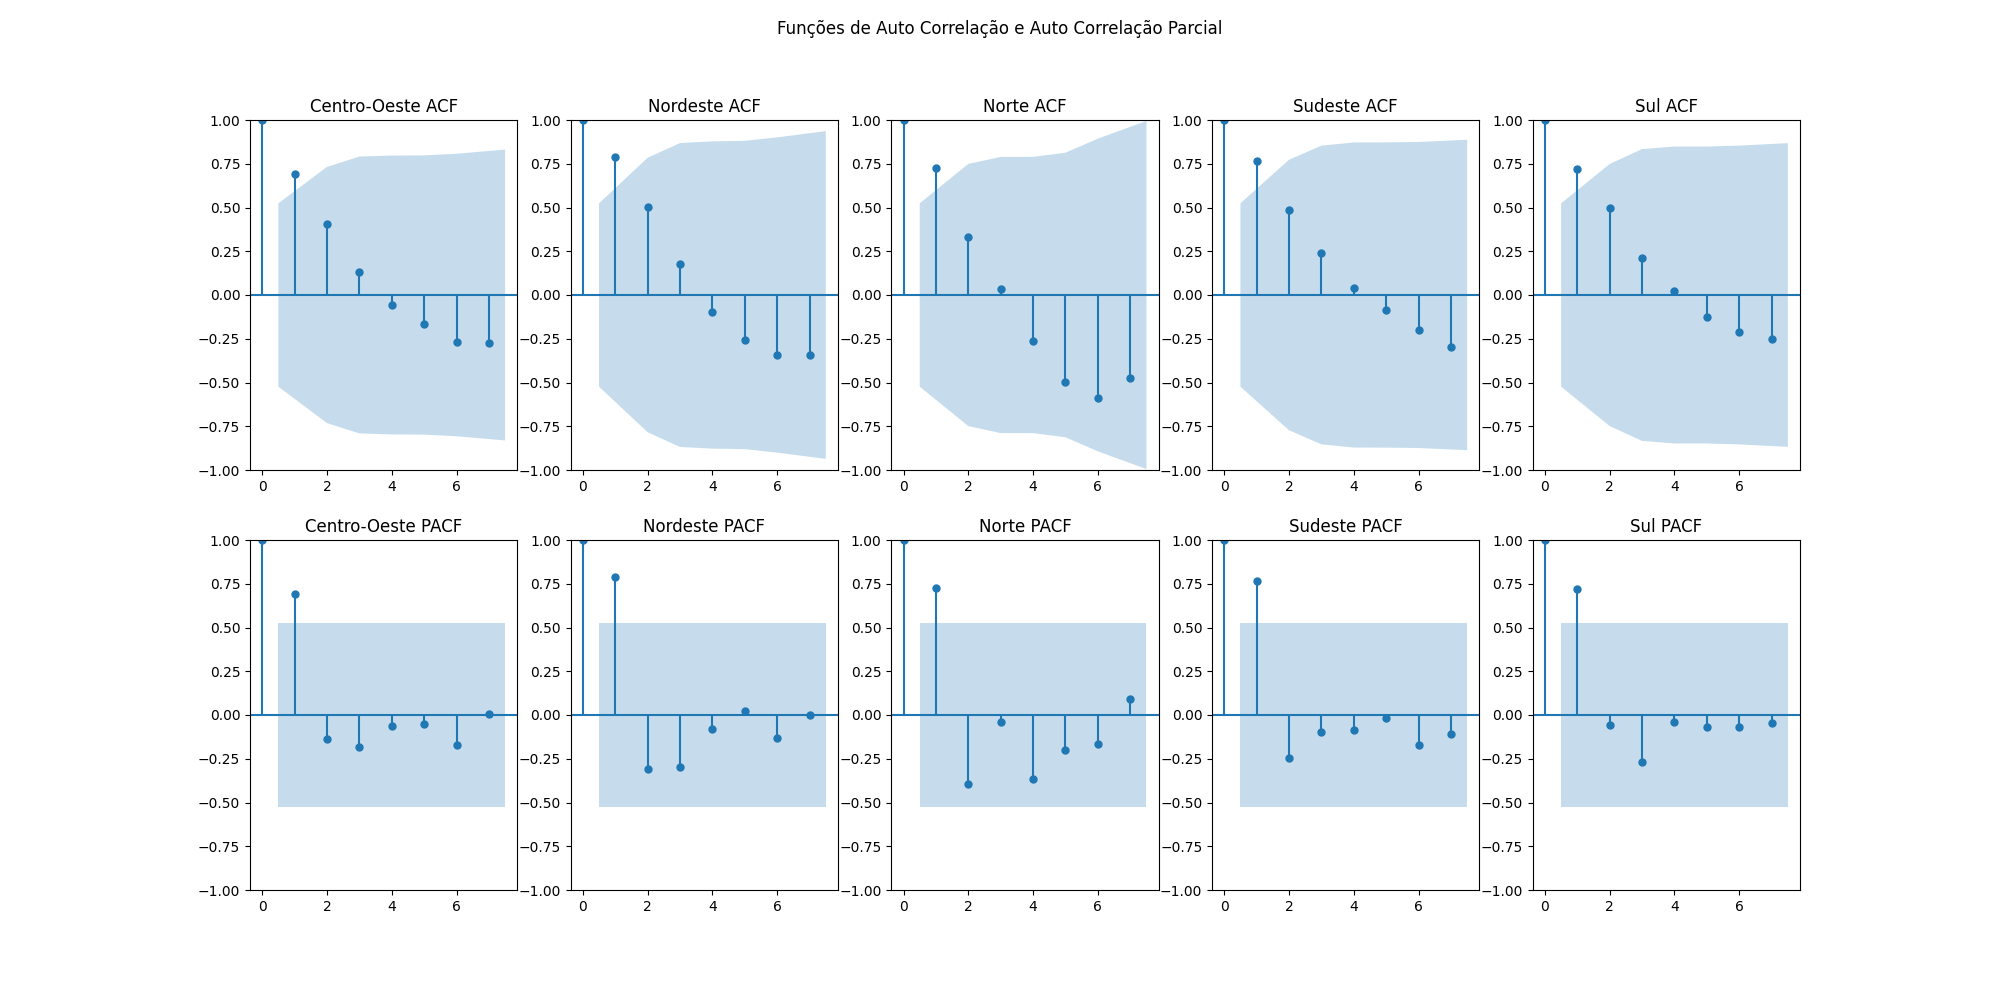
\includegraphics[width=\textwidth]{../figures/acf_pacf.png}
    \caption{\label{fig:corr} PACF e ACF para cada Grande Região do país.}
    \end{center}
\end{figure}

Quando lidamos com series temporais, uma das primeiras abordagens
é checar sua estacionaridade, para compreender quais técnicas são 
aplicáveis.

De acordo com a fígura \ref{fig:corr}, podemos perceber que a ACF 
decai gradualmente, o que indica que há algum tipo de tendência nos
dados. Além disso, a PACF só tem correlação significative com o primeiro lag,
evidenciando que somente a amostra imediatamente passada deve influenciar de
maneira consistente nossas predições. Cabe ressaltar que o ACF decai gradualmente
pois ele leva em conta as correlações acumuladas entre lags, já o PACF não. 

\begin{table}[h!]
\centering
\caption{\textit{Augmented Dickey–Fuller test}}
\label{tab:adf}
\begin{tabular}{ll}
\toprule
\textbf{Grande Região} & $\rho-\text{valor}$ \\
\midrule
Centro-Oeste  & 0.0719 \\
Nordeste  & 0.00515 \\
Norte  & 0.0411 \\
Sudeste & 0.000168 \\ 
Sul  & 0.167 \\
\bottomrule
\end{tabular}
\end{table}

Porém, de acordo com a Tabela \ref{tab:adf}, se supormos um nivel
de significância de $10\%$, todas as Grandes Regiões exceto a Sul passam no
teste, ou sejam, assumimos estacionaridade.

\label{ss:arima}
\subsection{Escolha do Modelo ARIMA}

A escolha do modelo ARIMA foi feita devido a baixa quantidade de dados e sua
simplicidade, pois é um modelo essencialmente linear.

A validação cruzada foi feita fazendo predições do futuro. Ou seja, treinei
o modelo para $N$ amostras e previa a $N+1$, após isso, o erro era avaliado.

Utilize a métrica de erro NRMSE, que é a raiz do erro quadrático médio
normalizada pelo desvio-padrão, devido a discrepância de escala dos nossos
dados.

\begin{equation}
    NRMSE = \frac{\sqrt{\frac{1}{N}\sum_{i=0}^{N} (y_i - \hat{y_i})^2}}{\sigma_x}
\end{equation}


\begin{table}[h!]
\centering
\caption{Melhores parâmetros de ordem ARIMA após validação cruzada}
\label{tab:arima_performance}
\begin{tabular}{lcccc}
\toprule
\textbf{Grande Região} & \textbf{NRMSE} & \textbf{Ordem AR} & \textbf{Ordem I} & \textbf{Ordem MA} \\
\midrule
Centro-Oeste  & 1.414 & 1 & 0 & 0 \\
Nordeste  & 0.503 & 1 & 0 & 0 \\
Norte  & 0.917 & 0 & 0 & 1 \\
Sudeste  & 1.651 & 0 & 1 & 0 \\
Sul  & 1.166 & 0 & 1 & 1 \\
\bottomrule
\end{tabular}
\end{table}

\begin{table}[h!]
\centering
\caption{Parâmetros da ordem mais estável}
\label{tab:arima_stable}
\begin{tabular}{lcccc}
\toprule
\textbf{Grande Região} & \textbf{NRMSE} & \textbf{Ordem AR} & \textbf{Ordem I} & \textbf{Ordem MA} \\
\midrule
Centro-Oeste  & 1.414 & 1 & 0 & 0 \\
Nordeste  & 0.503 & 1 & 0 & 0 \\
Norte  & 0.933 & 1 & 0 & 0 \\
Sudeste  & 1.651 & 1 & 0 & 0 \\
Sul  & 1.429 & 1 & 0 & 0 \\
\bottomrule
\end{tabular}
\end{table}

A partir da Tabela \ref{tab:arima_performance}, podemos ver que houve uma
discrepância entre qual ordem seria mais adequada a cada modelo. Alguns dos modelos
parecem ser estacionários, por assumir o parâmetro $i$ como 0.

Porém, ao analisarmos a Tabela \ref{tab:arima_stable}, que consta os dados da
ordem mais estável(i.e teve melhores resultados ao longo das regiões), que foi
um modelo AR(1), percebemos que a única região que apresentou baixa performance
para essa escolha foi a Sul, que foi a única região que o teste de
\textit{Dickey-Fuller} rejeitou a estacionaridade. Com isso, utilizaremos
modelos AR(1) para todas as regiões exceto a região Sul, que usaremos
ARIMA(0,1,1).

\section{Resultados} 

\subsection{Predição para os próximos dois anos} 

\begin{figure}[!htbp]
    \begin{center}
    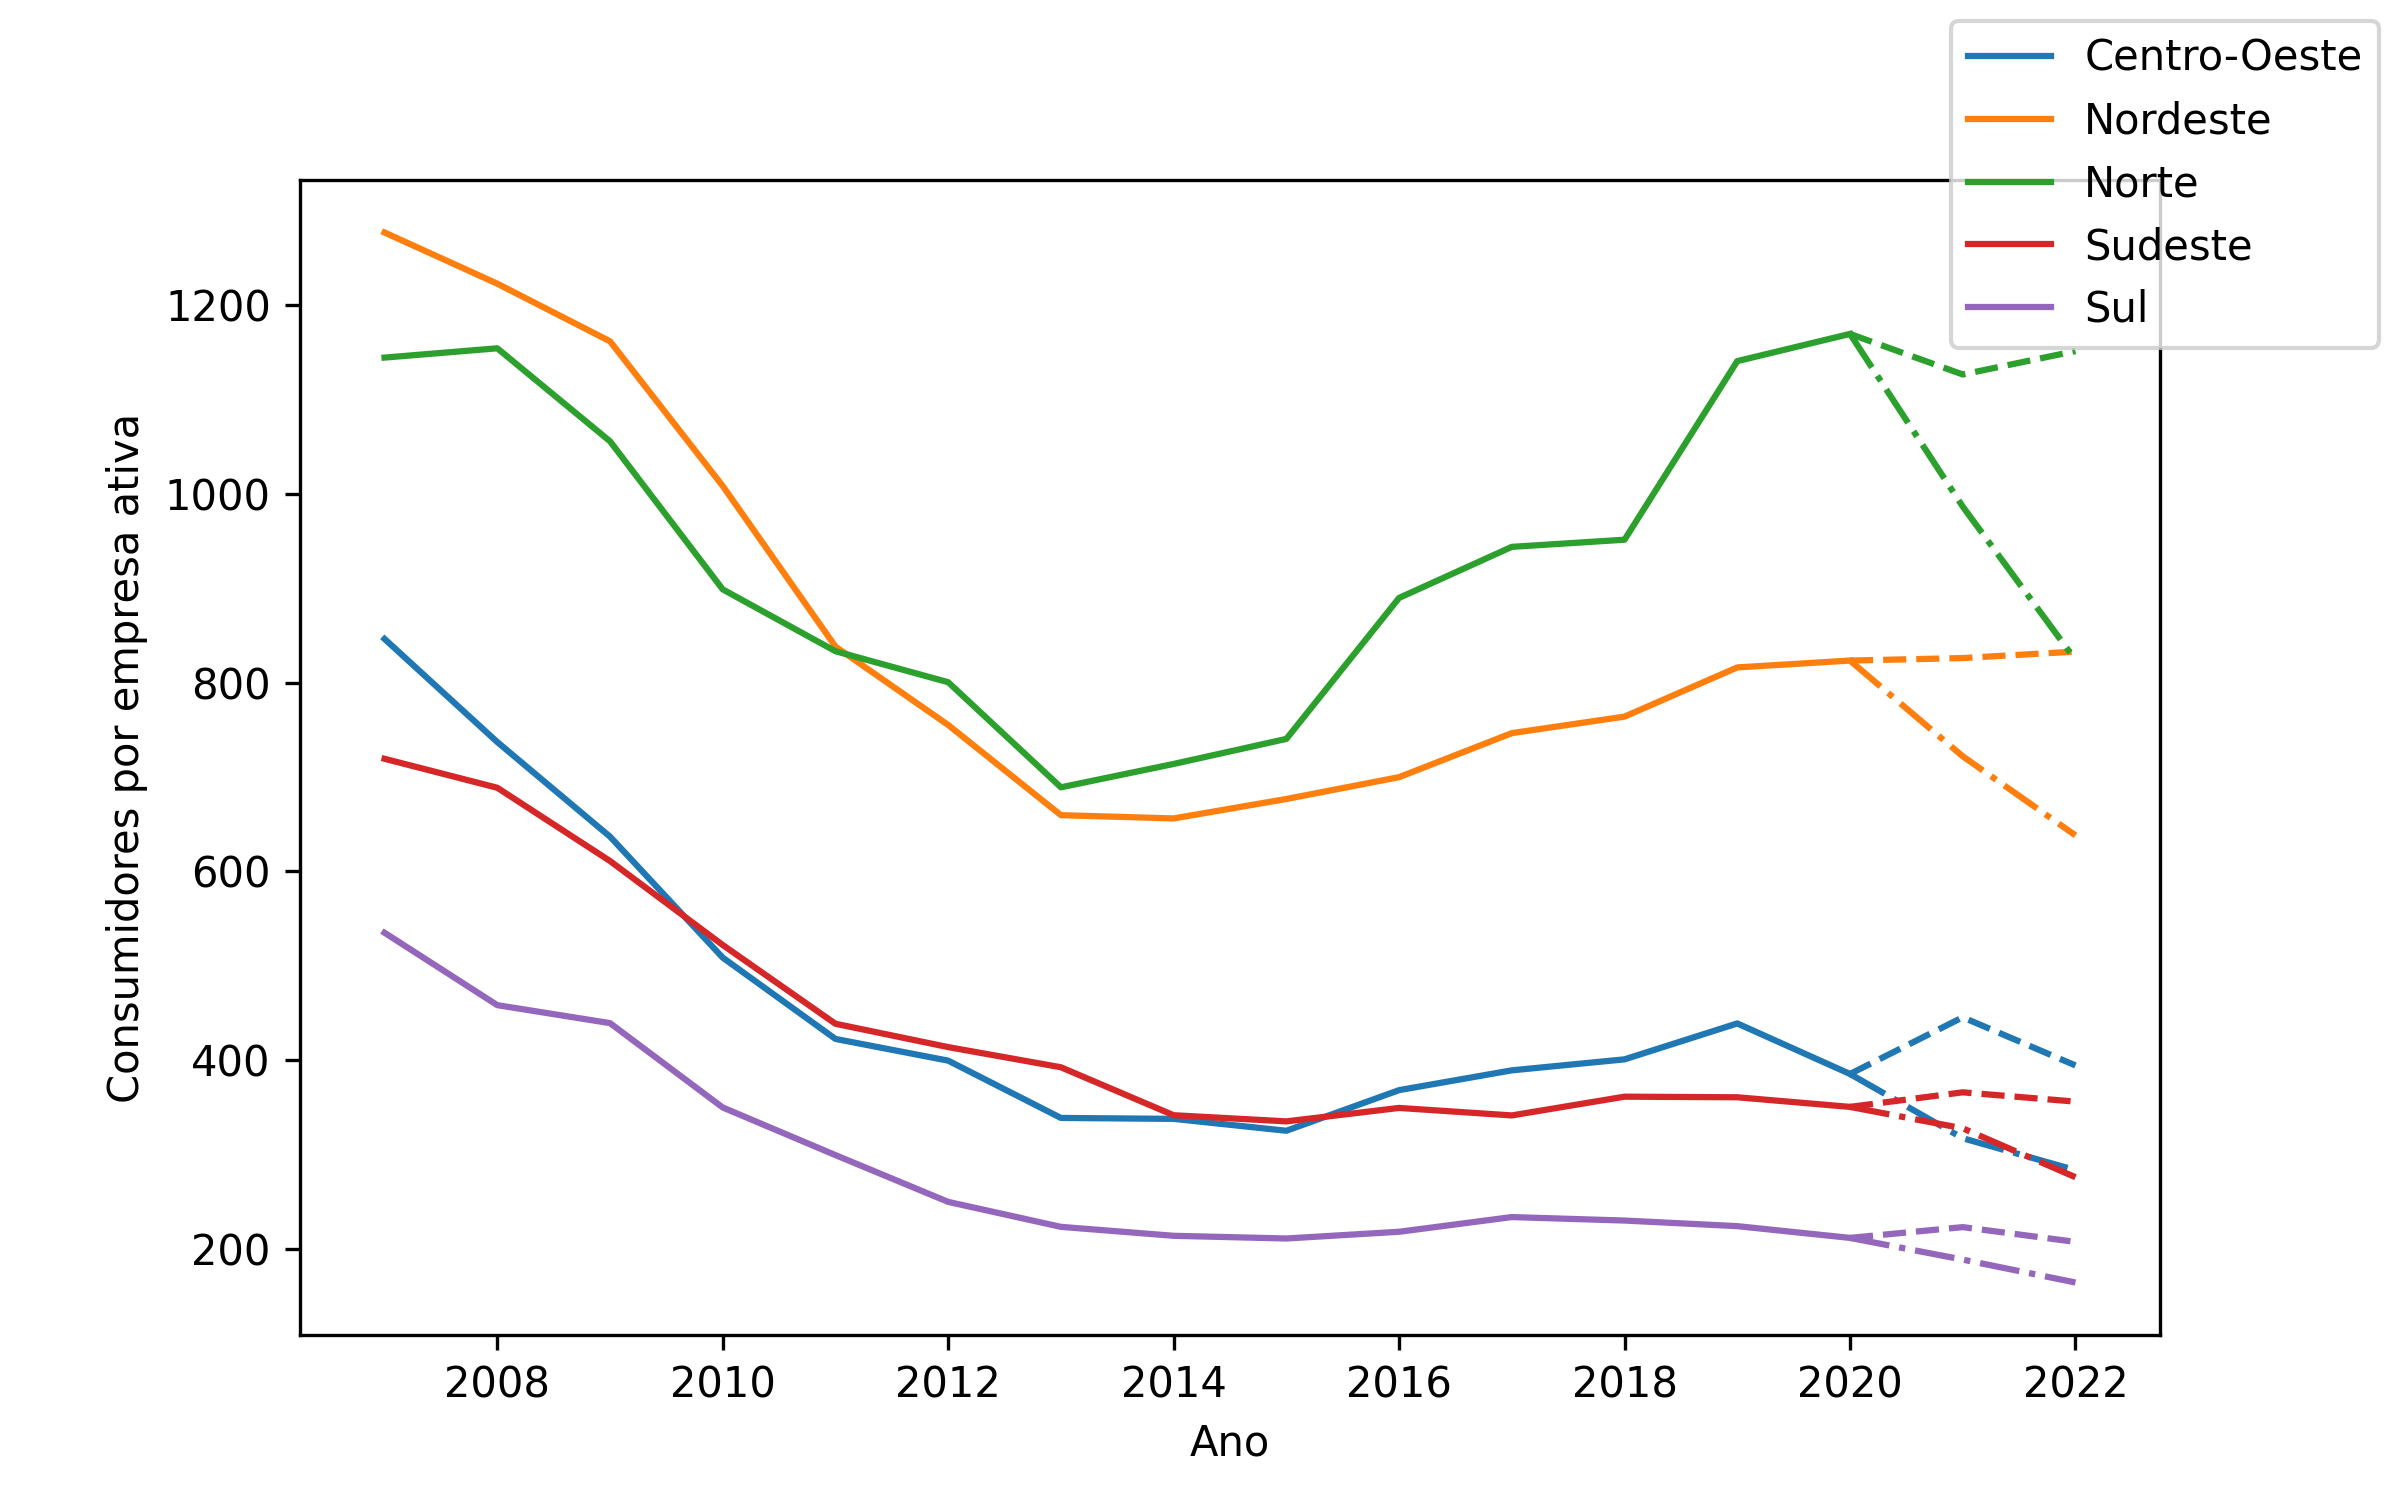
\includegraphics[width=0.7\textwidth]{../figures/forecast.png}
    \caption{\label{fig:forecast} Predição para os proximos dois anos}
    \begin{tikzpicture}
        \draw[black, thick] (0,0) -- (1,0) node[right]{Passado};
        \draw[black, thick, dashed] (0,-0.5) -- (1,-0.5) node[right]{Previsão};
        \draw[black, thick, dash dot] (0,-1) -- (1,-1) node[right]{Dados reais};
    \end{tikzpicture}
    \end{center}
\end{figure}

A Figura \ref{fig:forecast} mostra que o modelo apresentou um bom desempenho na
previsão dos anos analisados, com exceção de 2021 e 2022. Essa divergência não
indica uma falha do modelo, mas sim uma mudança abrupta nos dados devido à
pandemia, que alterou significativamente a dinâmica das empresas no Brasil.

Os dados do IBGE refletem a situação econômica no início de cada ano, o que
explica a baixa discrepância em 2020, já que a pandemia teve início no
Brasil apenas em março. No entanto, os anos seguintes registraram
oscilações atípicas na economia, tornando os padrões históricos menos
representativos e impactando a precisão das previsões.

Esses resultados reforçam que o modelo é confiável em condições normais, mas
eventos inesperados, como a pandemia, exigem abordagens complementares para
capturar seus efeitos nos dados.urados e Oportunidades

\subsection{Regiões Saturadas e Oportunidades}

A Figura \ref{fig:trend_rat} indica que as regiões Nordeste e Norte apresentam
grande potencial de crescimento, pois possuem uma alta proporção de
consumidores por empresa ativa, sugerindo baixa concorrência. Em contrapartida,
as regiões Sudeste e Centro-Oeste demonstram um nível maior de saturação, com
uma redução de aproximadamente 30\% nessa proporção. A situação é ainda mais
crítica na região Sul, que se destaca como a mais saturada, apresentando uma
queda de 50\% em relação às regiões com maior potencial de mercado.

\section{Conclusão} 

A performance de modelos de aprendizagem de máquina para predições de séries temporais
depende do contexto oferecido ao modelo. Não houve contexto suficiente para o
modelo tomar conclusões. Um dos contextos faltantes e dados correlatos é de uma
pandemia. Apesar disso, a performance do modelo ARIMA foi boa para os dados de
2007-2020, como mostrado na seção \ref{ss:arima}.

A pandemia introduziu variáveis atípicas no ambiente econômico, como
interrupções nas cadeias de suprimentos e mudanças no comportamento do
consumidor, que não estavam contempladas nos dados históricos utilizados para
treinar o modelo. Eventos inéditos como esse desafiam modelos preditivos,
resultando na queda da precisão das previsões nesses anos. Isso
destaca a necessidade de adaptar os modelos para lidar com situações
extraordinárias, garantindo previsões mais robustas em futuros cenários
voláteis.

Além disso, foi constatado que os mercados da região Norte e Nordeste são os com mais
oportunidades, mesmo após a queda abrupta causada pela pandemia.


\section*{Referências} 
\begin{itemize} 
    \item SCOD Brasil. Tendências do mercado
    imobiliário para 2023. Disponível em: \url{https://scod.com.br/blog/post/tendências-do-mercado-imobiliário-para-2023}
    \item IBGE. Tabela 1757 - Dados gerais das empresas de construção. Disponível em: \url{https://apisidra.ibge.gov.br/home/ajuda} 
    \item IBGE. Projeção da população. Disponível em: \url{https://www.ibge.gov.br/estatisticas/sociais/populacao/9109-projecao-da-populacao.html}
    \item Dickey, D.A. and W.A. Fuller (1979), “Distribution of the Estimators
        for Autoregressive Time Series with a Unit Root". Disponível em:
        \url{http://www.jstor.org/pss/2286348}. ” Journal of the American
        Statistical Association, 74, p. 427–431.
\end{itemize}

\end{document}
